\subsection{Les tests de base}

Les tests fournis passent tous avec succès dans l'implémentation dépourvue des
améliorations 'avancées' ainsi qu'avec la version utilisant plusieurs threads noyaux avec la fonction d'annulation des threads. 

Pour la version supportant les machines multiprocesseur, nous avons utilisé helgrind et drd le débogage et pour s'assurer du bon fonctionnement. Drd ne trouve rien de suspect mais helgrind nous prévient que l'ordre d'acquisition des mutex n'est pas toujours respecté. Nous pouvons sereinement ignorer cet avertissement car l'ensemble des programmes de tests ne souffrent pas de deadlock (vérifié avec l'option \verb!--exclusive-threshold! de drd où les seuls mutex pris longement sont ceux des threads en cours d'exécution, ce qui est normal) et le changement d'ordre d'acquisition des mutex est nécessaire pour notre méthode d'ordonnancement.

Nous avons également écrit un script pour tracer les courbes de performance
afin de pouvoir comparer graphiquement les temps d'exécution de notre
implémentation de threads utilisateurs lorsqu'on utilise les threads noyaux
et lorsqu'on ne les utilise pas.

\subsection{Tests implémentés}

\subsubsection{Les tris de tableaux} Les algorithmes de tri de tableaux $tri
rapide$ et $tri fusion$ ont été implémentés. Dans le cas du $tri rapide$
(fig. \ref{fig:quicksort}), un thread est créé et traite chaque partie du
tableau de part et d'autre du pivot. Pour le $tri fusion$
(fig. \ref{fig:mergesort}), chaque fois qu'un tableau est divisé en deux,
chaque partie est traitée par un nouveau thread.\\

%%%% resultats tests + include graphics %%%%
\begin{figure}[H]
\centering
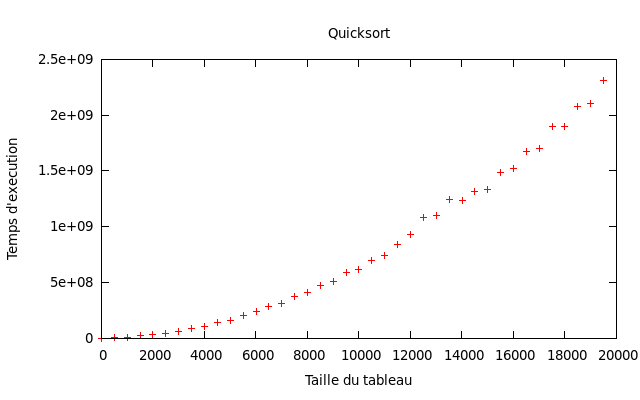
\includegraphics[width=0.9\textwidth]{figures/quicksort.png}
\caption{Temps d'exécution des tests d'un tri rapide}
\label{fig:quicksort}
\end{figure}

%%%% resultats tests + include graphics %%%%
\begin{figure}[H]
\centering
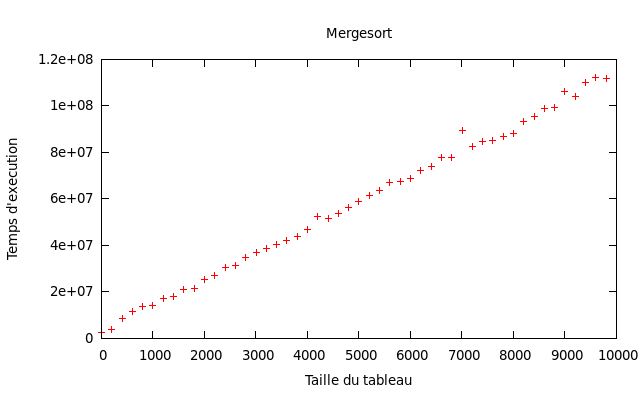
\includegraphics[width=0.9\textwidth]{figures/mergesort.png}
\caption{Temps d'exécution des tests d'un tri fusion}
\label{fig:mergesort}
\end{figure}

\subsubsection{Somme des éléments d'un tableau} Pour calculer la somme des
éléments d'un tableau (fig. \ref{fig:arraysum}), nous utilisons le même principe que pour le tri fusion,
à savoir diviser le tableau en deux et attribuer les deux parties à des threads
distincts. Une fois que l'on obtient des tableaux d'une case, leur valeur est
retournée et le thread parent calcule la somme des deux valeurs récupérées.

 %%%% resultats tests + include graphics %%%%
\begin{figure}[H]
\centering
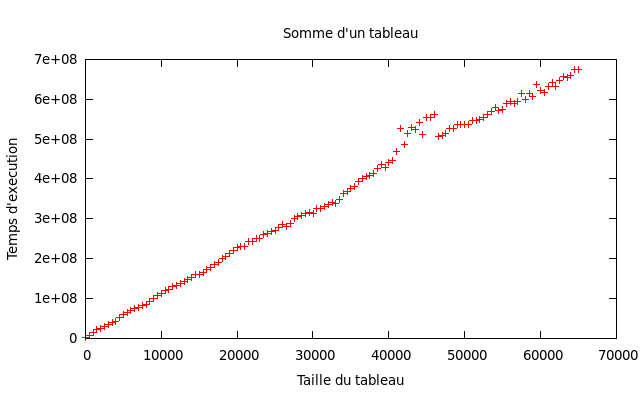
\includegraphics[width=0.9\textwidth]{figures/arraysum.png}
\caption{Temps d'exécution des tests sur la somme des éléments d'un tableau}
\label{fig:arraysum}
\end{figure}

\subsubsection{Incrémentation d'un entier avec threads noyaux}

Afin de vérifier que nos threads noyaux ont été correctement implémentés, nous
avons mis en place le test le plus basique possible. 4 threads utilisateurs
sont créés et chacun d'eux incrémentent un entier différent jusqu'à une valeur
définie par l'utilisateur. Ce test est ensuite lancé après avoir recompilé
notre code pour qu'il tourne sur $n$ processeurs ($n \in [1,4]$). On observe dans la
figure \ref{fig:comp-kthreads} les différences de temps d'exécution lorsqu'on
lance ce test sur un processeur ou sur quatre.

\begin{figure}[H]
\centering
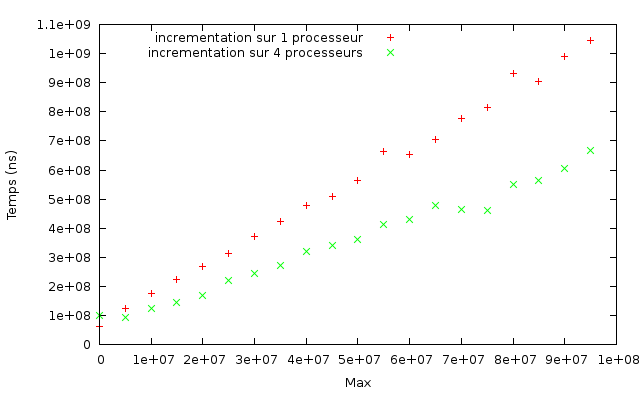
\includegraphics[width=0.9\textwidth]{figures/comparatif_kthreads.png}
\caption{Temps d'exécution des tests sur l'incrémentation d'un entier avec des
  threads noyaux}
\label{fig:comp-kthreads}
\end{figure}
